\chapter{Design}

\section{User Interface}
The first section, \textit{User Interface}, presents the designed four user interface. First, the four iterations and the changes between them are presented. Second, the final user interface design is discussed with usability heuristics by Nielsen and Apple.

\subsection{Iterations}
In this part, the different iterations of the user interface and their related think aloud protocol results are presented. The full user interface of each iteration can be seen in appendix \ref{appendix:userInterface}.

\paragraph{First Iteration}

The first iteration consist of five views. The application starts with the ''MapView - Loading'' view (cp Figure \ref{fig:i1-mv-loading}). The view shows a map on which the location of the users marked. At the top of the page a string indicates the current loading state of the system.

If the application fails to determine the parking position, a pop-up menu is shown (cp. Figure \ref{fig:i1-mv-error}) which notifies the user about the problem and explains the cause of the failure. 

On successful determination of the parking position, the view ''MapView - Determined Parking Postition'' (cf. Figure \ref{fig:i1-mv-parking}) is shown. It shows a map with the users location and the determined location of the users car. The label of the users car is clickable and opens ''MapView - Details''. 

''MapView - Details'' (cp. Figure \ref{fig:i1-mv-details}) presents more details about the determined parking position. It presents the address where the car is parked, the distance to the users car, the altitude difference between the user and the users car and the floor of the parked car. Two buttons are presented: One button opens a third party navigation software to navigate to the determined location, and a button to initiate reporting the accuracy of the determined parking position of the car by opening the ''Feedback'' view.

The ''Feedback'' (cp Figure \ref{fig:i1-feedback}) view presents the user instructions to report the accuracy of the determined parking position, the transmitted information and a button to report the information. When the button is clicked, the information is send and the application returns to the previous view, ''MapView - Details''. The user can also go back to the previous screen without sending any information by using the ''Back'' button.


The think aloud protocol shows two problems of the user interface. First, in the view ''MapView - Parking Position Determined'', the user does not understand that the car icon is clickable. Second, the user expects to be able to give feedback in text form in the ''Feedback'' view.

\paragraph{Second Iteration}

In the second iteration of the user interface, the two problems of the first iteration are improved. The views ''MapView - Details'' and ''MapView - Parking Position Determined'' are merged. This is done to present the user directly all details of the determined parking position. 
As the main view, ''MapView - Parking Position Determined'' (cp. Figure \ref{fig:i2-mv-parking}) now shows a partly transparent white box, this element is also added to the ''MapView - Loading'' view to keep the user interface consistent. It contains a button to initiate the determination of the car manually. 
In the new ''MapView - Parking Position Determined'' view, the call to action to give feedback is rephrased to ''Send accuracy'' to better represent the kind of feedback which can be given. The headline of the ''Feedback'' (cp. Figure \ref{fig:i2-feedback} view is changes accordingly. A pup up is introduced in the ''Feedback'' view to confirm the successfull sending of the accuracy.

The think aloud protocol of the second iteration shows three obstacles. First, the altitude in the view ''MapView - Parking Position Determined'' is understood as total altitude of the car, but it shows the relative altitude of the car compared to the current altitude of the user. Second, the user is unsure if the presented address the same view is the address of the location of the car but assumes so. Third, the user does not notice in the ''Feedback'' view that the accuracy is supposed to be reported at the actual parking position of the car.


\paragraph{Third iteration}

The third iteration improves on the three obstacles of the previous iteration. 
First, in the view ''MapView - Parking Position Determined'' (cp. Figure \ref{fig:i3-mv-parking}) the altitude information is split  into two rows. The row ''Relative Altitude'' shows the relative altitude between the users location and the cars location. The row ''Floor'' shows the floor of the determined parking location, if the data is available. Second, the headline ''Your car is parked at: '' is added to the view ''MapView - Parking Position Determined'' to clarify that the presented information are about the determined parking position. Third, a pop-up is introduced in the view ''Feedback'' (cp. Figure \ref{fig:i3-feedback-con}) to ensure the user is actually at the location of the parked car. 

The third iteration of the interface shows, that the call to action on the ''MapView - Parking Position Determined'' view is still not clear. The user is confused because the wording is unusual for giving feedback to improve an application.

\paragraph{Fourth Iteration}

To make the call to action to report the accuracy on the view ''MapView - Parking Position Determined'' (cf. Figure\ref{fig:i4-mv-parking}) ore clear, it is rephrased to ''Report accuracy''. The headline of the view ''Feedback'' (cf. Figure \ref{fig:i4-feedback}) is updated accordingly. To the view ''MapView - Parking Position Determined'' a small button is added to refresh the parking position of the car. 


In the four iterations of the user interface design, five design issues are removed. First, the call to action to send the accuracy is changed to ''Report Accuracy'' to make clear that no manual input is required and the user helps to evaluate the application. Second, the details of the determined parking location are made easier accessible by showing them as soon as the parking location is determined. Third, a confirmation dialog is introduced for the the reporting of the accuracy to ensure the user is at the location of their parked car. Fourth, a headline is introduced to clarify that the shown details are about the determined parking location. Fifth, the altitude data is presented in a clearer way by splitting the floor information and the altitude information into two rows and renaming ''Altitude'' to ''Relative Altitude'' to show that the altitude is relative to the users current location.


\subsection{Discussion of Final User Interface Design}

In the second part, \textit{Discussion of Final User Interface Design}, discusses the final user interface design. The different views are presented and and design decisions argued based on the user interface heuristics by Apple and Nielsen. \cite{nielsen1994usability} \cite{apple:interfaceguidliines}.

\paragraph{MapView - Loading}

\begin{figure}[h]
    \centering
    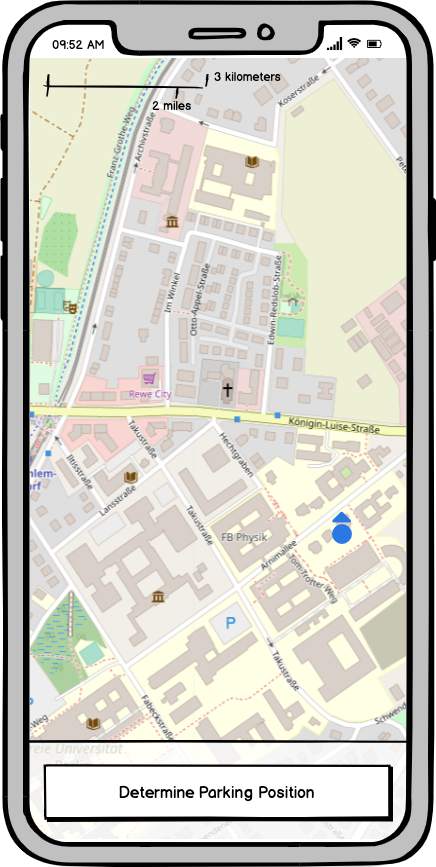
\includegraphics[width=0.4\textwidth]{images/UI/Iteration4-MapView-Loading.png}
    \caption{Map View - Loading}
    \label{fig:mv-loading}
\end{figure}

The application starts in the ''MapView - Loading'' view, shown in Figure \ref{fig:mv-loading}. The view consist of a map and a button to initiate the determination of the parking location of the users car. The show map supports the users to orientate themselves in their current environment by presenting their location on the map. Thus, the second heuristic from Nielsen, ''Match between system and the real world'', is implemented. The map is interactive and can be zoomed, moved and rotated. The button to determine the parking position of the users car is placed on top of a white and partly transparent box to ensure a sufficient contrast between the map and the button. The design fulfils Apples design guidelines for Maps. The basic design of a map with a white, partly transparent box is used for all of the apps views, except the ''Feedback'' view, to keep the design simple and consistent, according tho Nielsens fourth and eights heuristic. \cite{nielsen1994usability} \cite{apple:interfaceguidliines}


\paragraph{MapView - Error}

\begin{figure}[h]
    \centering
    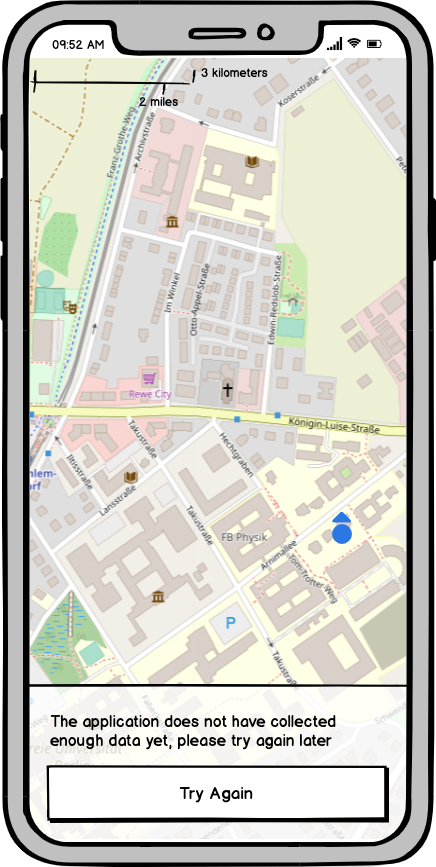
\includegraphics[width=0.4\textwidth]{images/UI/Iteration4-MapView-Error.png}
    \caption{Map View - Error}
    \label{fig:mv-error}
\end{figure}

If the application fails to determine the parking position of the users car, it shows the view ''MapView - Error'', shown in Figure \ref{fig:mv-error}. The view shows a map with the users location. On the bottom, an error message is printed on top of a white, partly transparent box. The error message explains in an understandable way for the users, why the application failed to determine the parking position. Below the error text, a button is shown. When pressed, the application tries to determine the parking position again. With the understandable error message and the promoted button to retry, the application confirms to Nielsens ninth heuristic, ''Help users recognize, diagnose, and recover from errors''. \cite{nielsen1994usability}

\paragraph{Map View - Parking Position Determined}

\begin{figure}[h]
    \centering
    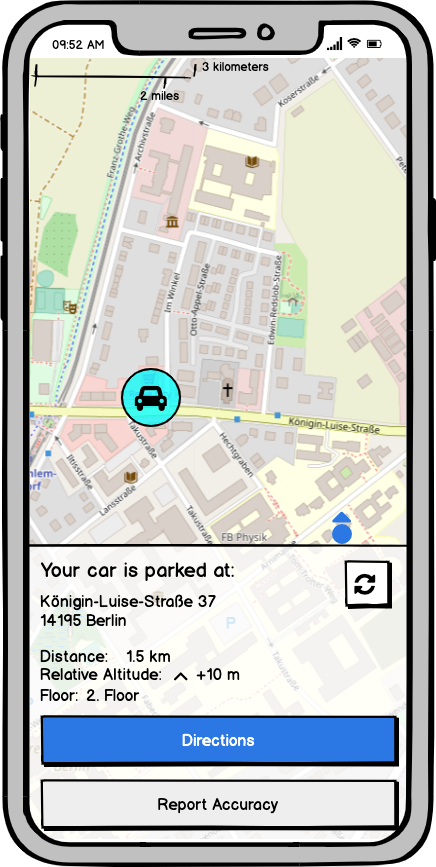
\includegraphics[width=0.4\textwidth]{images/UI/Iteration4-MapView-ParkingPositionDetermined.png}
    \caption{Map View - Parking Position Determined}
    \label{fig:mv-parking}
\end{figure}

The view ''Map View - Parking Position Determined'', shown in Figure \ref{fig:mv-parking}, is the main view of the application. It is shown when the application determined successfully the parking position of the users car. A map and a partly transparent white box is shown. On the map, the users current location and the position of the users car are marked. The users location is presented with a blue point with a blue triangle, pointing in the direction the user is headed. The location of the car is marked with a stylised car surrounded by a blue, transparent circle. The car icon is on the exact location, the application determined and the blue circle represents the accuracy of the determined parking location. The map view is chosen to match the system to the surroundings of the user. On the bottom of the screen, detailed information of the determined parking location are presented. The address, the distance to the current location, the relative altitude and the floor in which the car is parked are shown. Above the details the headline ''Your car is parked at'' clearly identifies the listed information as related yo the users car. Three buttons are shown. The first button, in the upper right corner of the white box, refreshed the determined parking location. The second button, labelled ''Directions'', opens a third party navigation software to navigate to the determined location. Because navigation apps, such as Apple Maps and Google Maps, use the color blue to indicate a button which starts a navigation, the color blue is also chosen for the ''Directions'' button. The third button, labeled ''Report Accuracy'', initiates the process of reporting the accuracy of the determined parking location. The refresh button and the ''Report Accuracy'' button are both colored white to not draw extra attention to them. Most users should not need to use them on a regular base. \cite{nielsen1994usability}


\paragraph{Feedback}


\begin{figure}[h]
  \centering
  \begin{minipage}[b]{0.49\textwidth}
    \centering
    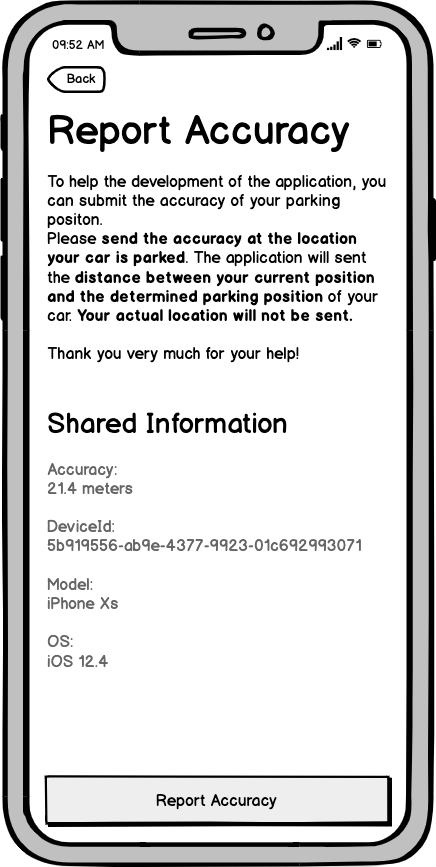
\includegraphics[width=0.6\textwidth]{images/UI/Iteration4-Feedback.png}
    \caption{Feedback}
    \label{fig:feedback}
  \end{minipage}
  \hfill
  \begin{minipage}[b]{0.49\textwidth}
    \centering
    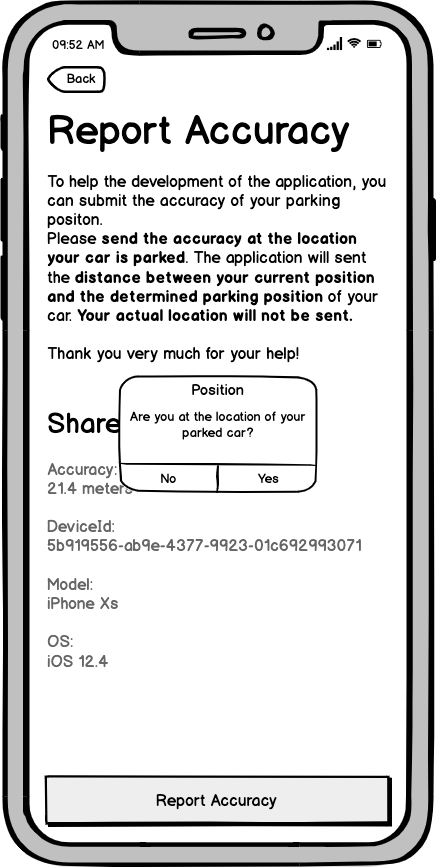
\includegraphics[width=0.6\textwidth]{images/UI/Iteration4-Feedback-Confirmation.png}
    \caption{Feedback - Confirmation}
    \label{fig:feedback-con}
  \end{minipage}
  
\end{figure}

The view ''Feedback'', shown in Figure \ref{fig:feedback}, enables the users to report the accuracy of the determined parking location. This functionality enables the quantitative evaluation of the systems accuracy. The text in the upper half of the screen explains how to report the accuracy and what kind of data is transmitted. A complete list of the to transmit data is shown in the bottom half. The ''Back'' button in the upper left corner navigates the system back to the view ''MapView - Parking Position Determined'' without transmitting any data. The button on the bottom, labelled ''Report Accuracy'', brings up a pop up in which the users are asked, if they are at the location of the parked car (cp. Figure \ref{fig:feedback-con}). User tests have shown that the instructions in the explaining text are often skimmed, thus this second check is necessary to keep the reported accuracy usable. If the user confirms their location, the data is send and a confirmation is shown (cf. Figure \ref{fig:feedback-succ}. The view changes back to the view ''MapView - Parking Position Determined''. If the user does not confirm their location, a pop up is shown (cp. Figure \ref{fig:feedback-fail}) which asks the user to report the accuracy at the location of their parked car. The ''Back'' button enables the user to be in control if they want to share any information. The confirmation dialog prevents users from accidental sending the accuracy at the wrong location. Thus, the view fulfills the third and fifth heuristic by Nielsen. \cite{nielsen1994usability}





\begin{figure}[h]
  \centering
  \hfill
  \begin{minipage}[b]{0.49\textwidth}
    \centering
    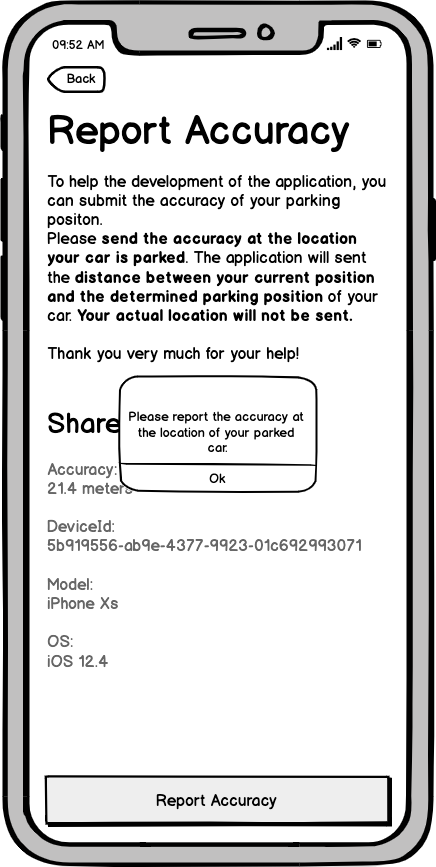
\includegraphics[width=0.6\textwidth]{images/UI/Iteration4-Feedback-Failure.png}
    \caption{Feedback - Failure}
    \label{fig:feedback-fail}
  \end{minipage}
  \hfill
  \begin{minipage}[b]{0.49\textwidth}
    \centering
    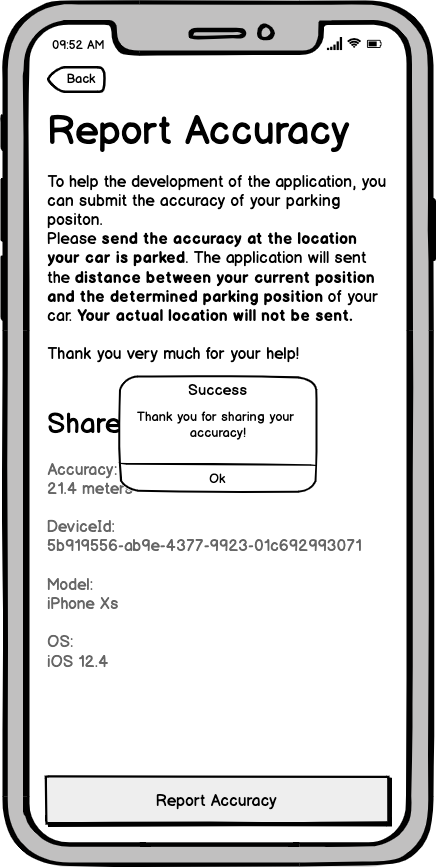
\includegraphics[width=0.6\textwidth]{images/UI/Iteration4-Feedback-Success.png}
    \caption{Feedback - Success}
    \label{fig:feedback-succ}
  \end{minipage}
\end{figure}

\section{Determining the location of the users car}
In the second section, \textit{Determining the location of the users car}, the approach to determine the location of the users car is described. The used transportation mode of the users spatial trajectory data is classified for a floating window of three segments. The parking position of the user is determined as the end point of the last significant stage with the transportation mode car.
The first section, \textit{Preprocessing}, describes the taken steps to clean and prepare the data of the geolife dataset.
The second section, \textit{Feature Extraction}, names and defines all features generated based on the geolife dataset.
The fifth section, \textit{Data Validation}, validates the generated data and drops all unplausable data.
The fourth section, \textit{Classification}, presents the uses machine learning model, XGBoost, and argues for its usage.
The fifth section, \textit{Parking Position Determination}, explains how the parking position of a users car is determined by using the transportation mode classification of the users spatial trajectory data.

\subsection{Preprocessing}
The first section, \textit{Preprocessing}, describes the taken steps to clean and prepare the data of the geolife dataset.

The geolife data set \cite{zheng2010geolife} \cite{zheng2008understanding} \cite{geolife-dataset} \cite{zheng2009mining} is created by Microsoft Research Asia in the context of the GeoLife project. It consist of spatial trajectories which are created by 182 users over five years. 69 of the users label their trajectories with the used transportation mode. The labels are saved in separate files. The labels have timestamps and needs to be joined to the trajectories. All trajectories without transportation mode labels are ignored.

To enable better access to the timestamp of the trajectories, the columns ''date'' and ''time'' are combined into one datetime column. All unused or redundant columns, such as ''date'', ''time'', and ''days\_total'' are dropped. As only the transportation modes ''car'', ''walk'', ''bike'', and ''train'' are used for classification, all rows with other transportation modes are dropped. 

The geolife dataset is joined with the transportation mode labels if possible. Then it is cleaned from unlabeled and unused rows and columns to be ready for the feature extraction. 

\subsection{Feature Extraction}
The second section, \textit{Feature Extraction}, names and defines all features generated based on the GeoLife dataset.

To enable the classification of the transportation mode, features are extracted from the GeoLife dataset. The classification is bases on a floating window set of three consecutive trajectory segments. Thus, all features are created based on three consecutive segments with the same transportation mode.

There are two kinds of features: First, individual features based on one single section, such as velocisty, acceleration and bearing change. Second, aggregated features based on a floating set of three segments. These are aggregations of the features individual to the segments, such as the minimum, the maximum, the range, the sum, the average, and the variance. In the following, the used features are defined.

\subsubsection{Individual Features}
The part \textit{Individual Features} describes the features that are generated for each individual segment. 

\paragraph{Velocity} The velocity of a trajectory is the movement speed of the tracked object. It is defined as $v(p_n) = Dist(p_n, p_{n+1})/(t(p_{n+1}) - t(p_n))$ with $Dist$ as a function to calculate the the distance between two coordinates and $t$ being the function that returns the timestamp of a point of a trajectory. \cite{Zheng2008}

\paragraph{Acceleration} The acceleration of a trajectory is the increase or decrease of speed in the given time. It is defines as $ a(p_n) = (v(p_{n+1}) - v(p_n))/(t(p_{n+1}) - t(p_n)$. \cite{Zheng2008}

\paragraph{Bearing Change} The bearing is the direction in which an object is heading in a spatial coordinate system. The bearing change is the absolute change of the bearing between two consecutive coordinates. It is defined as $ brCh(p_n) = 180 - | |brgn(p_n) - brng(p_{n+1})
| - 180| $ with $brng$ as the function that returns the bearing of the segment, defined as 
\begin{align*}
            y =& \sin (lon(p_{n+1})-lon(p_n)) \cdot \cos(lat(p_{n+1}) \\ 
            x =& \cos (lat(p_n)) \cdot \sin (lat(p_{n+1}))-\sin (lat(p_n))\\
               & \cdot \cos (lat(p_{n+1})) \cdot \cos(lon(p_{n+1})-lon(p_n)) \\
    brng(p_n) =& arctan(y,x)
\end{align*} \cite{Dabiri2018}

\subsubsection{Aggregated Features}
The part \textit{Aggregated Features} describes the funtions used to aggregate all features of the same kind of a floating window with three segments. As the functions are applied to all three individual features, the aggregation features are describes for the generic set $X$.

\paragraph{Maximum} The maximum of a set is the highest value in the set. It is defined as $ \max (X) = \max(x \in X)$.

\paragraph{Minimum} The minimum of a set is the lowest value in the set. It is defined as $ \min (X) = \min (x \in X) $.

\paragraph{Range} The range of a set is the difference between its minimum and its maximum. It is defined as $ range(X) = max(X) - min(X)$.  

\paragraph{Sum} The sum of a set is the sum of its elements. It is defined as $sum(X) = \sum_{x\in X} (x)$

\paragraph{Average} The average of a set is the mean value of the set. It is defined as $ avg (x) = sum(X)/|X|$.

\paragraph{Variance} The variance of a set it the squared deviation of the sets mean. It is defined as $var (X) = \sum_{x\in X} (x - avg(X))^2/|X| $.  

All aggregated features a generated for each kind of individual feature. Thus, for each sliding window with three segments, 9 individual features and 18 aggregated features are defined. 

\subsection{Data Validation}
% Data validation
The fifth section, \textit{Data Validation}, validates the generated data and drops all data that seems to be invalid.

To ensure no invalid data is used for the classification of the machine learning model, the data is cleaned using thresholds for speed and acceleration based on the transportation mode of the given set of segments. The thresholds are adapted from \cite{Dabiri2018} and can be seen in table \ref{table:thresholds}.
 
\begin{table}[h!]
    \centering
    \begin{tabular}{l l l l} 
     \hline
     Transportation mode & Maximum velocity ($m/s$) & maximum acceleration ($m/s^2$)\\
     \hline
     Walk & 7 & 3 \\
     Bike & 12 & 3 \\
     Car & 50 & 10 \\
     Train & 34 & 3 \\
     \hline
    \end{tabular}
    \caption{The used thresholds for velocity and acceleration \cite{Dabiri2018}}
    \label{table:thresholds}
\end{table}

All segments with a velocity or acceleration that extends the defined thresholds are dropped. 

\subsection{Classification}
The fourth section, \textit{Classification}, presents the uses machine learning model, XGBoost, and argues for its usage.

The used machine learning model is the XGBoost algorithm. XGBoost ''is an optimized distributed gradient boosting library designed to be highly efficient, flexible and portable''. The algorithm is used because it shows the best performance compared to other tree-based ensemble classifiers algorithms, such as Random Forest, Gradient Boosting Decision Tree and Support Vector Machine, and also compared to precious works that use other algorithms, such as \cite{Zheng2008} and \cite{dodge2009revealing}. \cite{Xiao2017} \cite{chen2016xgboost}

\subsection{Parking Position Determination}
The fifth section, \textit{Parking Position Determination}, explains how the parking position of a users car is determined by using the transportation mode classification of the users spatial trajectory data. 

To determine the parking position of the user car, the transportation mode of the most recent spatial trajectory data of the user is classified until a block of four consecutive sliding window sets are found that have ''car'' as their classified transportation mode. Four consecutive window sets are required to reduce the impact of false positive errors. The end point of the most recent segment form this set is defined as the parking position of the users car. 
